\chapter{The LHC and the CMS detector}
\ifpdf
    \graphicspath{{03_Detector/plots/}}
\else
    \graphicspath{{03_Detector/plots/EPS/}{03_Detector/plots/}}
\fi

\section{The Large Hadron Collider}
The LHC \cite{LHC} is currently the largest and the most powerful particle accelerator ever built. It is installed in
the 26.7 km tunnel that was originally constructed for the LEP accelerator in the 1980s. The tunnel lies at a depth of
45 m to 170 m underground between the Jura mountain and the Lake Geneva, being the main part of the CERN accelerator
complex.

The machine is designed to accelerate proton beams and provide collisions at a centre of mass energy of $\sqrt s = 14$
TeV. Unlike particle-antiparticle colliders, the LHC requires two rings with opposite magnetic dipole fields in order to
maintain and collide two counter-rotating proton beams. Since the tunnel was originally designed for the
electron-positron LEP, it has an internal diameter of 3.7 m which is not enough to install two separate independent
rings. Therefore, a twin-bore magnet design was adopted \cite{Blewett}, which also came as a substantial cost-saving
measure.

\begin{figure}[!htbp]
  \begin{center}
    \leavevmode
    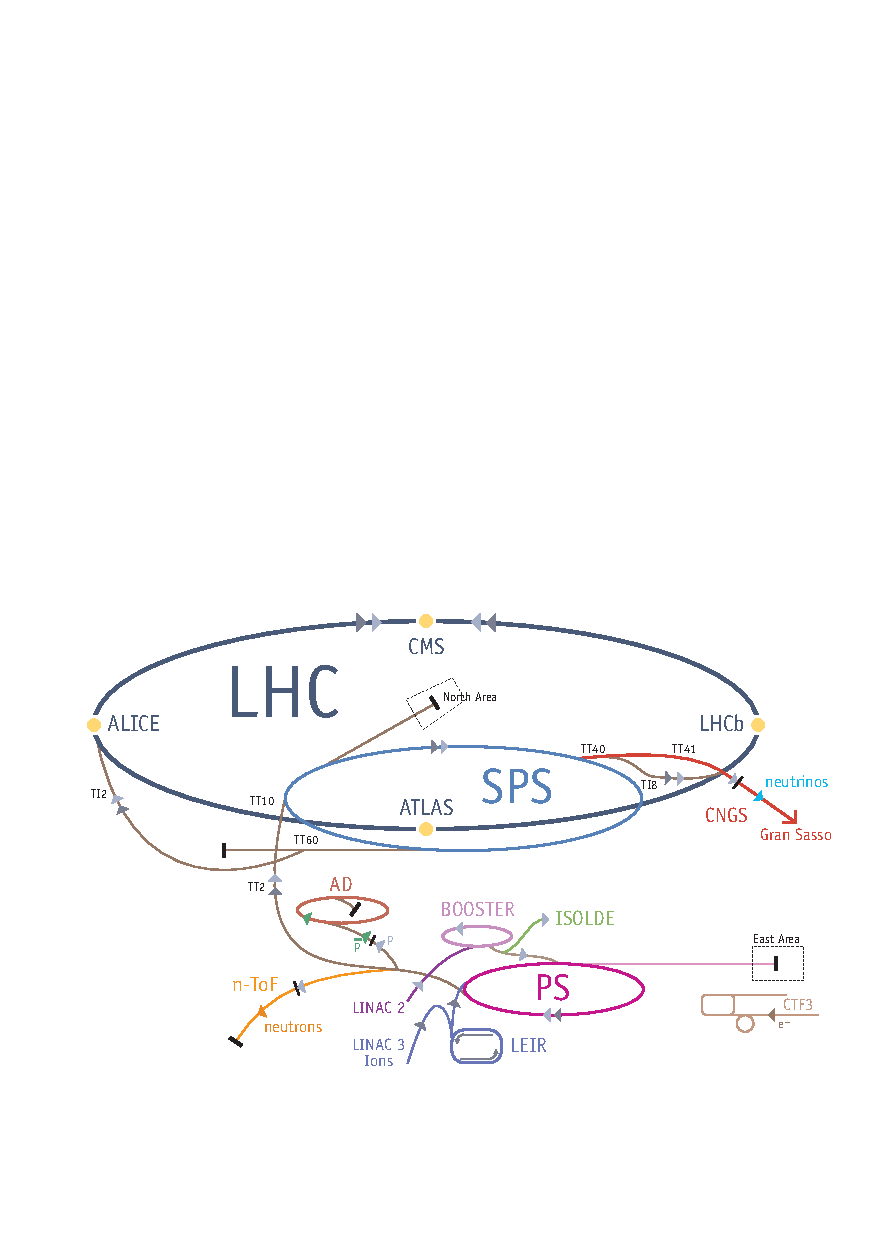
\includegraphics[width=\columnwidth]{LHC}
    \caption{CERN accelerator complex.}
    \label{LHC}
  \end{center}
\end{figure}

A schematic view of the LHC accelerator chain is shown on Figure~\ref{LHC}. In the beginning, the protons are obtained by
stripping orbiting electrons from hydrogen atoms. Then they are injected into the linear accelerator LINAC2 to reach the
energy of 50 MeV and enter the Proton Synchrotron Booster (PSB). The booster accelerates them to 1.4 GeV and passes the
beam to the Proton Synchrotron (PS) where the energy rises to 25 GeV. In the next step, protons enter the Super Proton
Synchrotron (SPS) where they are accelerated to 450 GeV. Finally, the beam is transferred to the LHC in both clockwise
and anti-clockwise directions where it takes about 20 minutes to reach the design 7 TeV energy (per beam).

\textit{[add the number of magnets, total energy stored, number of bunches, bunch spacing etc.?]}

The LHC has four interaction points, providing collisions to four major experiments. Two of them, CMS and ATLAS, are
multi-purpose high-luminosity experiments with a peak luminosity of $L = 10^{34}$ cm$^{-2}$ s$^{-1}$. The other two
experiments operate at low luminosities and have more specific physics goals: LHCb studies b-meson decays, and Alice is
a dedicated heavy ion experiment.

The instantaneous luminosity of a collider can be calculated as
\begin{equation}
	L = \frac{n_1 n_2 f}{4 \pi \sigma_x \sigma_y},
\end{equation}
where $n_1$ and $n_2$ are the numbers of particles in each of the colliding bunches, $f$ is the revolution frequency,
$\sigma_x$ and $\sigma_y$ are the horizontal and vertical beam sizes, assuming the two beams have the same size.

The number of events generated in the collisions per second is given by
\begin{equation}
	N_{events} = L \times \sigma,
\end{equation}

where $\sigma$ is the cross section of the process under study.

\textit{[add the plots with cross sections and production rates?]}

The LHC started operating on the 10th of September 2008, with the first beams fully circulating in both rings. However,
only 9 days later a magnet quench occurred in two sectors of the tunnel, which was caused by an electrical fault due to
a bad connection between two magnets. A consequent liquid helium explosion damaged a total of 53 superconducting
magnets. Over a year was spent on repairs and tests, and the first collisions were recorded on the 23rd of November 2009
at a centre of mass energy of 0.9 TeV. The following few months showed the continuous ramp up of the beam energies up to
3.5 TeV per beam which was achieved on the 30rd of March 2010 when the LHC physics program started.

Throughout the rest of the 2010 major LHC experiments (CMS and ATLAS) recorded approximately 40 pb$^{-1}$ of data,
which resulted in the first measurements of various physics processes at the LHC. The following year became the main 7
TeV data-taking period, with about 5 fb$^{-1}$ of data recorded by ATLAS and CMS. On the 5th of April 2012 the centre
of mass energy was increased to 8 TeV, and July of 2012 marked the first major discovery of a new boson which
was later shown to be consistent with the Standard Model Higgs boson, according to approximately 21.8
fb$^{-1}$ of data recorded until early 2013. A long shut-down is planned for the following two years with various
upgrades scheduled. The next physics run is expected in 2015 with the beam energy increased up to 6 or 7 TeV. 

\textit{[add any upgrade details and distant future plans, like SLHC?]}

\section{The CMS Detector}
The Compact Muon Solenoid \cite{CMS} is a general-purpose detector designed to carry out precise measurements of the
Standard Model and the searches for physics beyond it. The primary design requirement was the ability to
discover the nature of electroweak symmetry breaking, and the first observation of a Higgs boson was obtained in the
Summer of 2012 \cite{CMS_Higgs}.

The detector is installed at one of the LHC interaction points (Point 5) at about 100 m undeground near the French
village of Cessy, between the Jura mountains and Lake Geneva. The overall dimensions of the CMS detector are a length of
21.6 m, a diameter of 14.6 m and a total weight of 12500 tons.

\begin{figure}[htbp]
  \begin{center}
    \leavevmode
    \includegraphics[width=\columnwidth]{CMS}
    \caption{Sectional view of the CMS detector.}
    \label{CMS}
  \end{center}
\end{figure}

The sectional view of CMS is shown on Figure~\ref{CMS}. In the centre of the detector, tracking and calorimetry systems
are surrounded by the superconducting solenoid. On the outermost part of it the magnetic flux is returned through the
iron yoke in which the muon system is also integrated. All the sub-systems are discussed in the following sections with
more detail.

The cylindrical shape of the CMS detector dictates using the cylindrical coordinate system, with the origin centered at
the interaction point, the $x$-axis pointing towards the centre of the LHC ring, the $y$-axis pointing upwards and the
$z$-axis pointing along the beamline in the anti-clockwise direction. The azimuthal angle $\phi$ is measured from the
$x$-axis in the transverse ($x-y$) plane and the polar angle $\theta$ is measured from the $z$-axis. Tha radial distance
to the beamline is denoted as $r$. Pseudorapidity is defined as:
\begin{equation}
  \eta = - \ln{\tan{\frac{\theta}{2}}}.
\end{equation}
This implies that the particles moving in the transverse plane (perpendicular to the beamline) have a pseudorapidity of
0, whereas the beam direction has an infinite pseudorapidity. Considering the cylindrical shape of the detector, it has
the barrel and the endcaps regions, with the transition occuring at $\eta = 1.4$. The momentum and energy transverse to
the beamline are denoted by $p_T$ and $E_T$ respectively; the imbalance of the energy measured in the transverse plane,
called missing transverse energy, is denoted by \ETm.

\subsection{Inner Tracking System}
The tracking system lies in the heart of the CMS detector and is the closest to the interaction point where the particle
flux has the highest value. This determines high requirements on the configuration of the system. At design luminosity
of $L = 10^{34}$ cm$^{-2}$ s$^{-1}$ with the bunch spacing of 25 ns, an average of 1000 particles from about 25
proton-proton interactions (pile-up vertices) is expected to traverse the tracker for each bunch crossing. However, up
until the long shutdown the bunch spacing of 50 ns was used, which meant the higher number of protons in each bunch
leading to approximately twice as higher number of pile-up vertices. Therefore, in order for the particle tracks to be
identified reliably and separately for each bunch crossing, the tracker requires a very fine granularity and fast
response parameters. Another complication caused by the intense particle flux is the severe radiation damage, so the
tracker has to be highly resilient in operating in the harsh environment for a reasonable lifetime.

To meet these requirements on granularity, response time and radiation resilience, the tracker design was chosen to be
based on silicon detector technology. Although capable to meet such conditions, this technology has a disadvantage of a
high power density of on-detector electronics. This implies the necessity of an efficient cooling system. Moreover, a
large amount of dense material interacting with the particles leads to the higher multiple scattering, bremsstrahlung,
photon conversions and nuclear interactions. Therefore, there are complications in the reconstruction of the tracks,
meaning some loss of efficiency and precision. This will be discussed in detail later on in the object reconstruction
section.

\begin{figure}[htbp]
  \begin{center}
    \leavevmode
    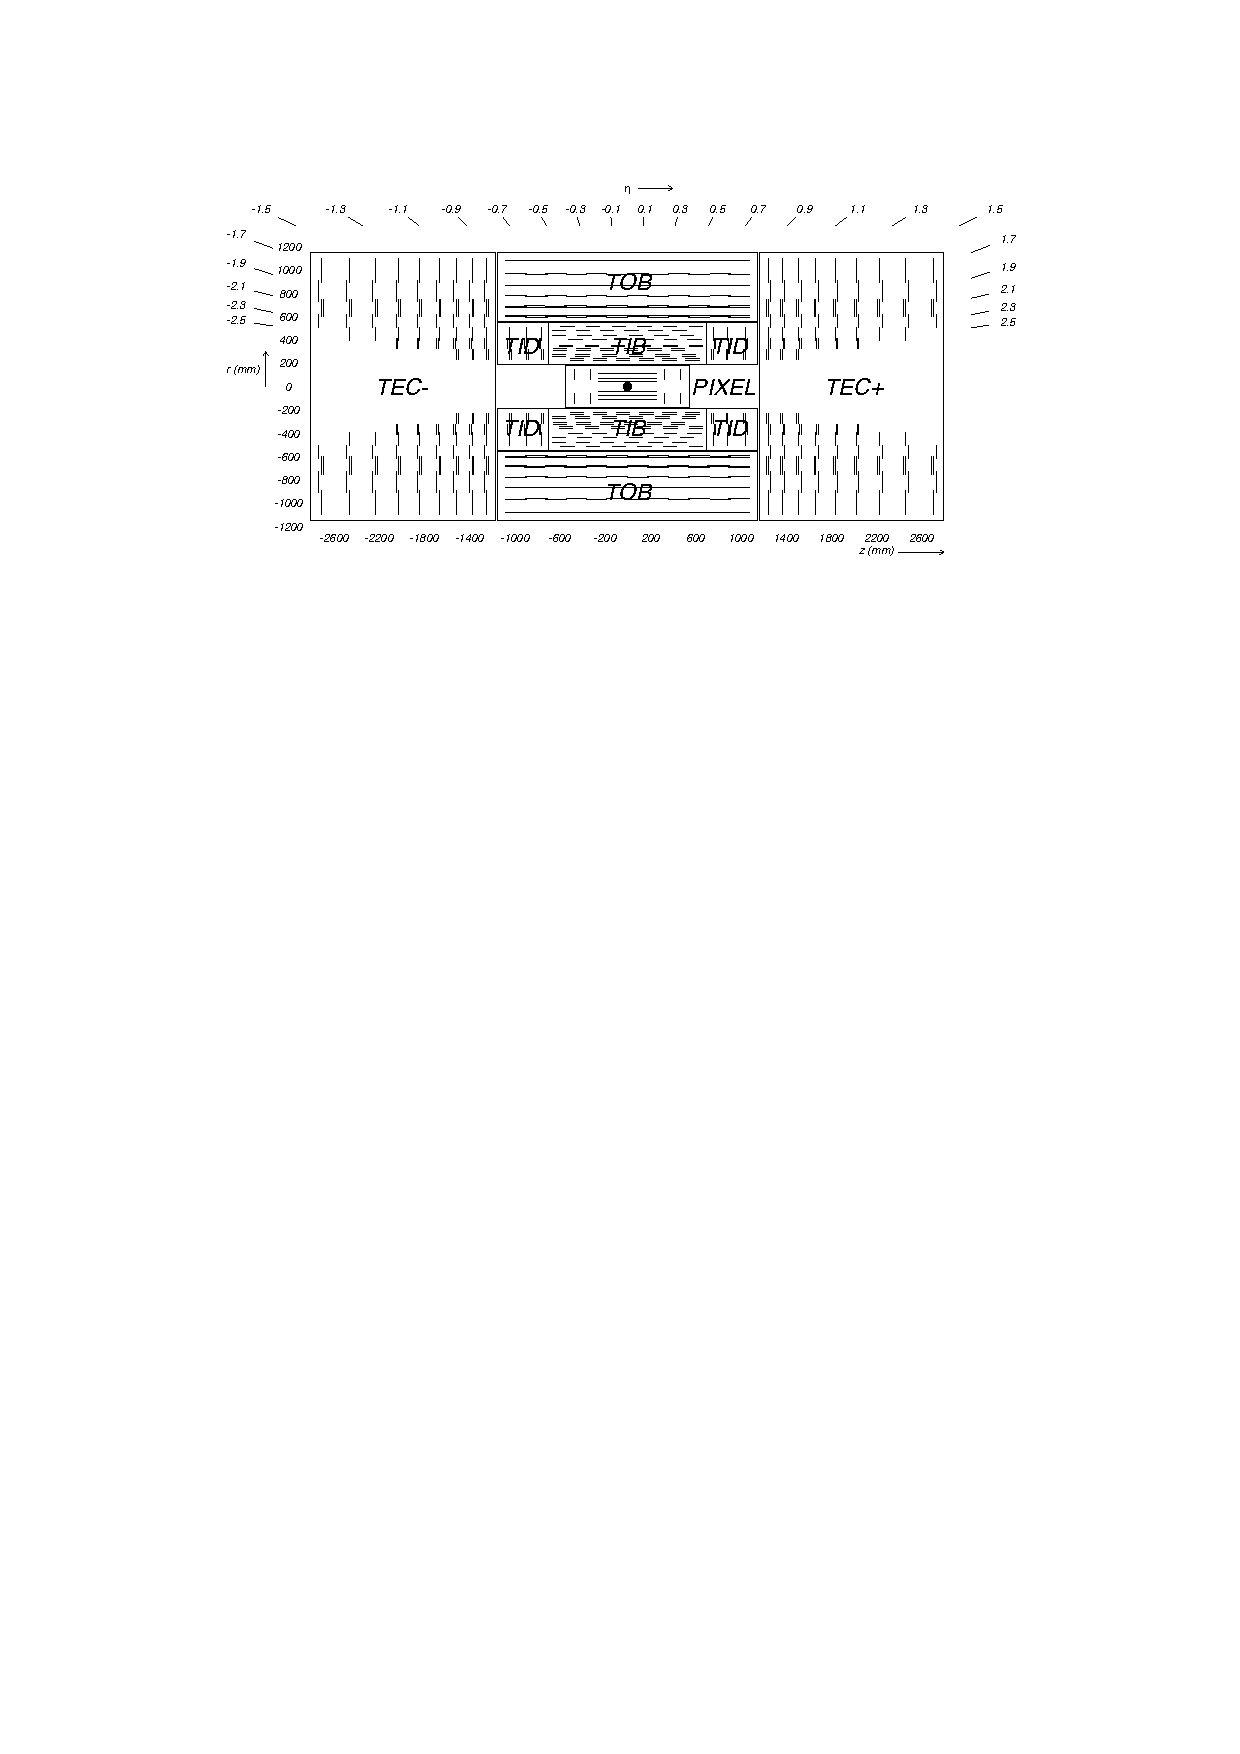
\includegraphics[width=\columnwidth]{tracker}
    \caption{Cross-section of the CMS tracker system.}
    \label{Tracker}
  \end{center}
\end{figure}

Figure~\ref{Tracker} shows the overall layout of the tracking system. It consists of the inner pixel detector, located
in the vicinity of the interaction point, and silicon strip tracker detectors: inner barrel and disks (TIB and TID),
outer barrel (TOB) and endcaps (TEC). The geometrical acceptance of the tracker system goes up to \abs\eta $<2.5$. The
outer radius of the CMS tracker reaches approximately 110 cm, and its total length is about 540 cm.

The pixel detector consists of three layers of pixel sensors at radii of 4.4 cm, 7.3 cm and 10.2 cm from the beamline in
the barrel region. In addition there are two endcap disks on each side at \abs z $=$ 34.5 cm and 46.5 cm. The pixel size
equals $100 \times 150~\mu m^2$ in $r \phi \times z$ coordinates. The pixel detector has 66 million pixels and the total
area of about 1 $m^2$.

The silicon strip tracker consists of the several layers of the silicon microstrip detectors. It covers the region
between 20 to 110 cm in radius and extends up to $\pm$ 280 cm in the z direction. The Tracker Inner Barrel (TIB) is made
out of 4 layers and the Tracker Outer Barrel (TOB) has 6 layers in it. The tracker endcaps (TEC) comprise 9 disks, and
there are also the tracker inner disks (TID) that consist of 3 discs filling the gap between TIB and TEC. There are 9.3
million silicon strips covering the area of about 200 $m^2$. The silicon sensors' thickness varies between 320
and 500 $\mu m$ and the strip pitch varies from 80 $\mu m$ in the TIB to 180 $\mu m$ in TOB and TEC.

\subsection{Electromagnetic Calorimeter}

\subsection{Hadron Calorimeter}

\subsection{Superconducting Magnet}

\subsection{Muon System}

\subsection{Trigger and Data Acquisition}
[1.4 experimental challenge in TDR]

\section{Computing}

\section{Object Reconstruction}

\subsection{Electron Reconstruction}

\subsection{Muon Reconstruction}

\subsection{Jet Reconstruction}

\subsection{Missing Transverse Energy}

\section{Summary}

% ------------------------------------------------------------------------

%%% Local Variables: 
%%% mode: latex
%%% TeX-master: "../thesis"
%%% End: 
